\section{Proofs of Section~\ref{sec:mvica}}
\label{sec:app_proofs}
\subsection{Proof of Prop.~\ref{prop:identifiability}}
\label{app:proof:mvica:identifiability}
We fix a subject $i$. Since $\sbb$ has independent components, so does $\sbb + \nb_i$. Following~\cite{comon1994independent},
Theorem 11, there exists a scale-permutation matrix $P^i$ such that $A'_i =
A_iP^i$. As a consequence, we have $\sbb  + \nb_i = P^i(\sbb' + \nb'^i)$ for all
$i$.

Then, we focus on subject 1 and subject $i \neq 1$:
\begin{align}
  &\sbb + \nb^1 - (\sbb + \nb_i) = P^1(\sbb' + \nb'^1) - P^i(\sbb' + \nb'^i)\\
  &\nb^1 - \nb_i = P^1(\sbb' + \nb'^1) - P^i(\sbb' + \nb'^i)\\
  &\iff P^1\sbb' - P^i\sbb' = P^i \nb'^i - \nb_i + \nb^1 - P^1 \nb'^1 \label{eq:condition_Gaussian}
\end{align}
% This shows that $P^1\sbb' - P^i\sbb'$ is Gaussian which can only happen if $P^1= P^i$. 
Since the right hand side of equation (\ref{eq:condition_Gaussian}) is a linear combination of Gaussian random variables, this would imply that $P^1\sbb' - P^i\sbb'$ is also Gaussian. However, given that $\sbb'$ is assumed to be non-Gaussian, the equality can only hold if $P^1
= P^i$ and both the right and the left hand side vanish.
Therefore, the matrices $P^i$ are all equal, and there exists a scale and permutation matrix $P$ such that $A'_i = A_iP$.

\subsection{Proof of Prop.~\ref{prop:robust}}
\label{ref:robust}
We consider $W_i = \Lambda (A_i)^{-1}$, where $\Lambda$ is a diagonal matrix.
%
We recall $\xb_i= A_i (\sbb + \nb_i),$ so that $\yb_i = W_i\xb_i= \Lambda(\sbb + \nb_i)$.
%
The gradient of $\loss$ is given by equation~\eqref{eq:gradient}:
\begin{align*}
  \mathcal{G}^i &= \frac{1}{m}f'(\tilde{\sbb})(\sbb + \nb_i)^{\top}\Lambda \\ & \enspace \enspace+ \frac{1 - 1/m}{\sigma^2} \Lambda\left(\nb_i - \frac{1}{m-1}\sum_{j\neq i} \nb^j\right)(\sbb + \nb_i)^{\top}\Lambda - I_p \\
  & = \frac{1}{m}f'(\Lambda(\sbb + \frac1m\sum_j\nb^j))(\sbb+\nb_i)^{\top} \Lambda + \frac{\sigma'^2(1 - 1/m)}{\sigma^2} \Lambda^2 - I_p
    \numberthis
\end{align*}
where we write $f'(\sbb) = \begin{bmatrix}f'(s_1) \\ \vdots \\ f'(s_p) \end{bmatrix}$.
Therefore, $\mathcal{G}^i$ is diagonal and constant across subjects (because $f'(\Lambda(\sbb + \frac1m\sum_j\nb^j))(\nb_i)^{\top} = f'(\Lambda(\sbb + \frac1m\sum_j\nb^j))(\nb^{i'})^{\top}$).
Let us therefore consider only its coefficient $(a, a)$, and let $\lambda = \Lambda_{aa}$:
$$
\mathcal{G}^i_{aa} =G(\lambda) = \phi(\lambda)\lambda + \frac{\sigma'^2(1 - 1/m)}{\sigma^2}\lambda^2 - 1,
$$
where $\phi(\lambda) = \frac{1}{m}f'(\lambda(s_a + \frac1m\sum_j n^j_a))(s_a+n_a^i)$. One the one hand, we have $G(0) = -1$. On the other hand, if we assume for instance that $f'$ has sub linear growth (i.e. $|f'(x)| \leq c|x|^{\alpha} +d$ for some $\alpha < 1$) or that $\phi$ is positive, we find that $G(+\infty) = +\infty$.
Therefore, $G$ cancels, which concludes the proof.

\subsection{Stability conditions}
\label{sec:stability}
We consider $W_i = \Lambda (A_i)^{-1}$ where $\Lambda$ is such that the gradients $\mathcal{G}^i$ all cancel. We consider a small relative perturbation of $W_i $ of the form $W_i \leftarrow (I_p + E^i)W_i$, and consider the effect on the gradient.
We define $\Delta^i=\mathcal{G}^i\left((I_p + E^1)W_1, \dots, (I_p + E^m)W_m\right)$.
Denoting $C = \frac{1 - 1/ m}{\sigma^2}$ and $\tilde{\nb} = \frac1m\sum_{i=1}^m \nb_i$, we find:
\begin{align*}
  \Delta^i = \Delta^i_1 + C\Delta^i_2 - I_p
\end{align*}

where
\begin{align*}
     &\Delta^i_1= \\&\frac1m f'\left(\Lambda(\sbb + \tilde{\nb}) + \frac1m \sum_{j=1}^m E^j\Lambda(\sbb +\nb^j)\right)(\sbb +\nb_i)^{\top}\Lambda(I_p + E^i)^{\top} \numberthis
 \end{align*}
 and
 \begin{align*}
   &\Delta^i_2= \left(\Lambda\nb_i - \frac{1}{m-1}\sum_{j\neq i} \Lambda\nbb^j + E^i\Lambda(\sbb + \nb_i) \right. \\& \left. - \frac{1}{m-1}\sum_{j\neq i} E^j \Lambda(\sbb + \nb^j)\right)(\sbb + \nb_i)^{\top}\Lambda(I_p + E^i)^{\top}
   \numberthis
\end{align*}

The first term is expanded at the first order, denoting $S = \sum_{j=1}^m E^j$:

\begin{align*}
  \Delta_1^i &= \frac1m \Bigg( f''(\Lambda(\sbb + \tilde{\nb}))\odot \big(\frac1m \sum_{j=1}^m E^j\Lambda(\sbb +\nb^j)\big) \\& + f'(\Lambda(\sbb + \tilde{\nb})) \Bigg) (\sbb +\nb_i)^{\top}\Lambda(I_p + E^i)^{\top}\\
    &=\frac1m f'(\Lambda(\sbb + \tilde{\nb}))(\sbb + \nb_i)^{\top}\Lambda(I_p + E^i)^{\top} \\&+ \frac1{m^2}S\odot  \left(f''(\Lambda(\sbb + \tilde{\nb}))(\sbb^2)^{\top}\Lambda^2 \right)\\
    &+\frac{1}{m^2}E^i\odot\left(f''(\Lambda(\sbb + \tilde{\nb}))((\nb_i)^2)^{\top}\Lambda^2 \right)
      \numberthis
\end{align*}
The symbol $\odot$ denotes the element-wise multiplication, $f'(\sbb) = \begin{bmatrix}f'(s_1) \\ \vdots \\ f'(s_p) \end{bmatrix}$ and $f''(\sbb) = \begin{bmatrix}f''(s_1) \\ \vdots \\ f''(s_p) \end{bmatrix}$.
Similarly, the second term gives at the first order: 
\begin{align}
    \Delta_2^i &= \sigma'^2\Lambda^2(I_p + E^i)^{\top} + (1 + \sigma'^2)E^i\Lambda^2 - \frac{1}{m-1} (S - E^i) \Lambda^2
\end{align}

Combining this, we find:

\begin{align}
 \Delta^i = (E^i)^{\top} + E^i \odot\Gamma^E
 +S\odot \Gamma^S
\end{align}
where 
$$
\Gamma^E= \left(\frac1{m^2}f''(\Lambda(\sbb + \tilde{\nb}))((\nb_i)^2)^{\top} + (1-\frac1m)\frac{\sigma'^2}{\sigma^2} + \frac{1}{\sigma^2} \right)\Lambda^2
$$
$$
\Gamma^S =\left(\frac1{m^2}f''(\Lambda(\sbb + \tilde{\nb}))(\sbb^2)^{\top} -\frac{1}{m\sigma^2}  \right)\Lambda^2
$$

are $p\times p$ matrices, independent of the subject.
This linear operator is the Hessian block corresponding to the $i$-th subject:
Denoting $\mathcal{H}$ the Hessian, it is the mapping $\mathcal{H}(E^1, \dots, E^m) = (\Delta^1, \dots, \Delta^m)$.

The coefficient $\Delta^i_{ab}$ only depends on $(E^i_{ab}, E^i_{ba}, E^1_{ab},\dots, E^m_{ab})$. Therefore, the Hessian is block diagonal with respect to the blocks of coordinates $(E^1_{ab}, E^1_{ba}, \dots, E^m_{ab}, E^m_{ba})$. Denote $\varepsilon = \Gamma^E_{ab}$, $\varepsilon' = \Gamma^E_{ba}$, $\beta = \Gamma^S_{ab}$ and $\beta'= \Gamma^S_{ba}$. The linear operator for the block is:

\begin{align*}
&K(\varepsilon, \varepsilon', \beta, \beta')= \\
&\left(
    \begin{array}{ll|ll|l|ll}
\varepsilon + \beta & 1       & \beta & 0       & \dots  & \beta & 0       \\
1      & \varepsilon' + \beta' & 0      & \beta' & \dots  & 0      & \beta' \\
\hline
\beta & 0       & \varepsilon + \beta & 1       &        & \beta & 0       \\
0      & \beta' & 1      & \varepsilon' + \beta' & \ddots & 0      & \beta' \\
\hline
\vdots & \vdots  &        & \ddots  & \ddots & \vdots & \vdots  \\
\hline
\beta & 0       & \beta & 0       & \dots  & \varepsilon + \beta & 1       \\
0      & \beta' & 0      & \beta' & \dots  & 1      & \varepsilon' + \beta'
    \end{array}
\right)
\end{align*}
The positivity of $\mathcal{H}$ is equivalent to the positivity of this operator for all pairs $a, b$.
We now assume $\beta \beta' > 0$.

First, we should note that $K(\varepsilon, \varepsilon', \beta, \beta') $ is
congruent to $K(\varepsilon \sqrt{\frac{\beta'}{\beta}}, \varepsilon'
\sqrt{\frac{\beta}{\beta'}}, \sqrt{\beta\beta'}, \sqrt{\beta\beta'})$ via the
basis \\ $\text{diag}((\frac{\beta'}{\beta})^{1/4}, (\frac{\beta}{\beta'})^{1/4}, \cdots,(\frac{\beta'}{\beta})^{1/4}, (\frac{\beta}{\beta'})^{1/4})$.
%
We denote to simplify notation $\alpha = \varepsilon \sqrt{\frac{\beta'}{\beta}}$, $\alpha' = \varepsilon' \sqrt{\frac{\beta}{\beta'}}$ and $\gamma = \sqrt{\beta\beta'}$. We only have to study the positivity of $K(\alpha, \alpha', \gamma, \gamma)$.
We have:
$$
K(\alpha, \alpha', \gamma, \gamma) =  I_m  \otimes M_\alpha+ \gamma  \mathbb{1}\otimes I_2, \enspace M_\alpha = 
\begin{pmatrix}
\alpha & 1 \\
1 & \alpha'
\end{pmatrix}
$$
Since $I_m\otimes M_\alpha$ and $\gamma \mathbb{1}\otimes I_2$ commute, the minimum value of $\text{Sp}(K)$ is $\text{min}(I_m\otimes M_\alpha) + \text{min}(\gamma\text{Sp}(\mathbb{1}))=\frac12(\alpha + \alpha' - \sqrt{(\alpha - \alpha')^2 + 4}) + m\min(0, \gamma)$.
Since we assumed $\beta \beta' > 0$ we have $\gamma > 0$. This is similar to the usual ICA case, we find that the condition is $\alpha\alpha' > 1$.

If the following conditions hold for all pair of components $a, b$, the components are a local minimum of the cost function:
\begin{itemize}
    \item $\Gamma^S_{ab}\Gamma^S_{ba}\geq 0$
    \item $\Gamma^E_{ab}\Gamma^E_{ba} > 1$
\end{itemize}
% \section{Identifiability for Shared Response Model}
% \label{sec:app_identifiability}
% The shared response model~\cite{chen2015reduced} (SRM) models the data $\xb_i \in \bbR^v$ of subject $i$ for $i = 1,\dots, m$ as
% \begin{align*}
%     \xb_i = A_i \sbb + \nb_i \enspace \text{with} \enspace \sbb \sim \Ncal(0, \Sigma), \enspace\nb_i \sim \Ncal(0, \rho_i^2 I_v), \enspace {A_i}^{\top}A_i = I_p
% \end{align*}
% where $A_i \in \bbR^{v, k}$, $\sbb \in \bbR^p$ and  $\Sigma \in \mathbb{R}^{k, k}$ is a symmetric positive definite matrix.

% \begin{proposition}
% SRM is not identifiable
% \end{proposition}
% \begin{proof}
% Let us assume the data $\xb_i \enspace i=1, \dots, m$ follow the SRM model with parameters $\Sigma, A_i, \rho_i^2 \enspace i=1, \dots, m$. 

% Let us consider an orthogonal matrix $O \in \Ocal_k$.
% We call $A'_i = A_i O$ and $\Sigma' = O^{\top} \Sigma O$. 
% $\Sigma'$ is trivially symmetric positive definite.

% Then the data also follows the SRM model with different parameters $\Sigma', A'_i, \rho_i^2 \enspace i=1, \dots, m$.
% \end{proof}

% \begin{proposition}
% We consider the decorrelated SRM model with an additional decorrelation assumption on the shared responses.
% \begin{align*}
% \xb_i = A_i \sbb + \nb_i \enspace \text{with} \enspace \sbb \sim \Ncal(0, \Sigma), \enspace\nb_i \sim \Ncal(0, \rho_i^2 I_v), \enspace {A_i}^{\top}A_i = I_p
% \end{align*}
% where $\Sigma$ is a positive \emph{diagonal} matrix. We further assume that the values in $\Sigma$ are all distinct and ranked in ascending order.
% The decorrelated SRM is identifiable up to sign indeterminacies on the columns of 
% $\begin{bmatrix}
% A_1 \\
% \vdots \\
% A_m
% \end{bmatrix}
% $.
% \end{proposition}
% \begin{proof}
% The decorrelated SRM model can be written
% \begin{align*}
%     &\xb_i \sim \Ncal(0, A_i \Sigma {A_i}^{\top} + \rho_i^2 I_v) \enspace \text{with}\enspace  {A_i}^{\top}A_i = I_p
% \end{align*}
% where $\Sigma$ is a positive diagonal matrix with distincts values ranked in ascending order.

% Let us assume the data $\xb_i \enspace i=1, \dots, m$ follow the decorrelated SRM model with parameters $\Sigma, A_i, {\rho_i}^2 \enspace i=1, \dots, m$. Let us further assume that the data $\xb_i \enspace i=1, \dots, m$ follow the decorrelated SRM model with an other set of parameters $\Sigma', A'_i, {\rho'_i}^2 \enspace i=1, \dots, m$.

% Since the model is Gaussian, we look at the covariances.
% We have for $i \neq j$
% \begin{align*}
%     \bbE[\xb_i\left(\xb_j\right)^{\top}] = A_i\Sigma {A_j}^{\top} = A'_i \Sigma'{A'_j}^{\top} \enspace, 
% \end{align*}
% The singular value decomposition is unique up to sign flips and permutation. Since eigenvalues are positive and ranked the only indeterminacies left are on the eigenvectors. For each eigenvalue a sign flip can occur simultaneously on the corresponding left and right eigenvector.

% Therefore we have $\Sigma' = \Sigma$, $A_i = A'_i D_{ij}$ and $A_j = A'_j D_{ij}$ where $D_{ij} \in \bbR^{k, k}$ is a diagonal matrix with values in $\{-1, 1\}$. This analysis holds for every $j \neq i$ and therefore $D_{ij} = D$ is the same for all subjects.

% We also have for all $i$
% \begin{align*}
%     \bbE[\xb_i \left(\xb_i\right)^{\top}] = A_i \Sigma {A_i}^{\top} + \rho_i^2 I_v =  A'_i \Sigma' {A'_i}^{\top}  + {\rho'}_i^2 I_v\\
% \end{align*}
% We therefore conclude ${\rho'}_i^2 = \rho_i^2, i=1 \dots m$.

% Note that if the diagonal subject specific noise covariance $\rho_i^2 I_v$ is replaced by any positive definite matrix, the model still enjoys identifiability.
% \end{proof}

\subsection{Reproducing time-segment matching experiment}
\label{appendix_reproduce}
[Omitted long matching line]

The results are available in Figure~\ref{fig:supp_timesegment}.

\begin{figure}
  \centering
  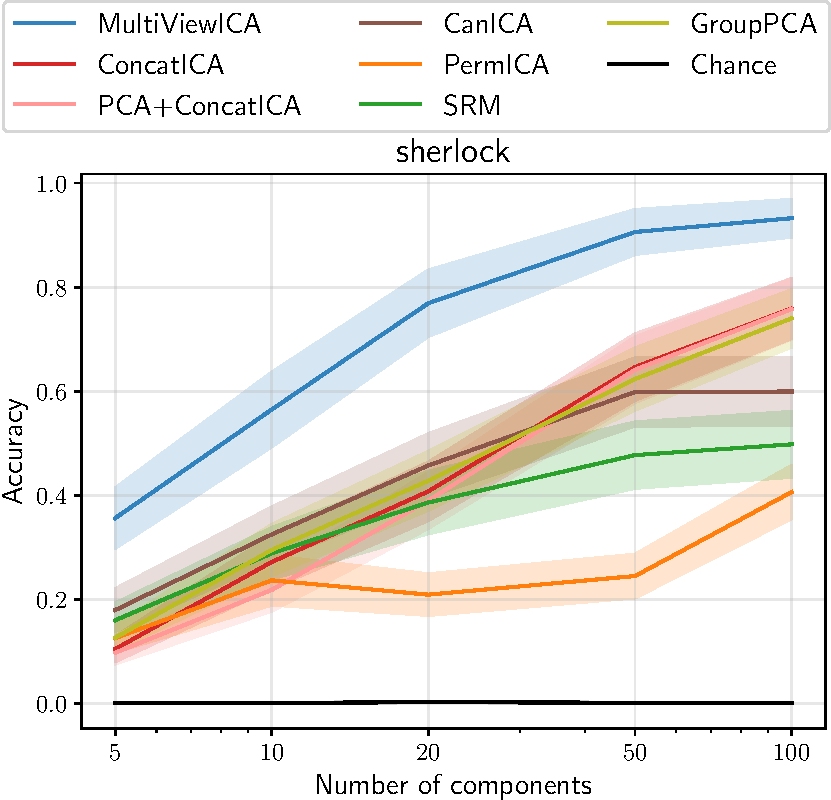
\includegraphics[width=0.6\textwidth]{figures/mvica/timesegment_matching_cae.pdf}
  \caption{\textbf{Reproducing the time-segment matching experiment of \cite{chen2016convolutional}~\cite{zhang2016searchlight}} Mean classification accuracy - error bars represent 95\% confidence interval}
  \label{fig:supp_timesegment}
\end{figure}

\section{Related Work}
\label{sec:app_rel_work}
The following table describes some usual method for extracting shared components from multiple subjects datasets.
The column "Modality/Components" describes the type of data for which each algorithm was \emph{initially} proposed, even though each algorithm could be applied on any type of data. 
%
The components type can be either temporal if extracted components are time courses or spatial if they are spatial patterns. 
%
\begin{center}
\begin{longtable}{ |p{.2\textwidth} | p{.21\textwidth} |p{.2\textwidth}| p{.24\textwidth}|}
\hline
\textbf{Method} & \textbf{Modality / Components} &\textbf{Dimension reduction} & \textbf{Description}  \\
\hline
SRM \cite{chen2015reduced} & 
fMRI/Temporal
&
SRM
&
The model is $\xb_i = A_i\sbb + \nb_i$, with \emph{Gaussian} components and \emph{orthogonal} mixing matrices $A_i$\\
\hline
GroupPCA~\cite{smith2014group} &
fMRI/Spatial
&
GroupPCA
&
A memory efficient implementation of PCA applied on temporally concatenated data.\\
\hline
GIFT~ \cite{calhoun2001method} & 
fMRI/Spatial
&
Individual PCA + Group PCA (on component-wise concatenated data)
&
Single-subject ICA is applied on the aggregated data\\
\hline
EEGIFT~ \cite{eichele2011eegift} & 
EEG/Temporal
&
Individual PCA + Group PCA (on component-wise concatenated data)
&
Single-subject ICA is applied on the aggregated data\\
\hline
PermICA &
Any
&
Any
&
Single-subject ICA is applied on each subject's data, and the components are matched using the Hungarian algorithm\\
\hline
Clustering approach~\cite{esposito2005independent}&
fMRI/Spatial
&
Individual PCA
&
Single-subject ICA is applied on each subject's data, and the components are matched using a hierarchical clustering algorithm.\\
\hline
Measure projection analysis~\cite{bigdely2013measure}&
EEG/Temporal
&
Individual PCA
&
Single-subject ICA is applied on each subject's data, and the components are matched using a hierarchical clustering algorithm.\\
\hline
TensorICA \cite{beckmann2005tensorial} &
fMRI/Spatial
&
Group PCA (on spatially concatenated data)
&
TensorICA incorporates ICA assumptions into the PARAFAC model. The mixing matrices $A_1 \cdots A_n$ are such that $A_i = A D_i$ where $A$ is common to all subjects and $D_i$ are subject specific diagonal matrices.\\  
\hline
Unifying Approach of \cite{guo2008unified} &
fMRI/Spatial
&
Group PCA (on spatially concatenated data) + GroupPCA (on component-wise concatenated data).
&
The model is $\xb_i = A_i\sbb + \nb_i$ with a Gaussian mixture model on independent components and a matrix normal prior on the noise. \\
\hline
SR-ICA \cite{zhang2016searchlight} &
fMRI/Temporal
&
SR-ICA
&
SR-ICA incorporates ICA assumptions into the shared response model.  \\
\hline
CAE-SRM \cite{chen2016convolutional}
&
fMRI/Temporal
&
CAE-SRM
&
A convolutional auto-encoder is used to perform the unmixing. \\  
\hline
CanICA \cite{varoquaux2009canica} &
fMRI/Spatial
&
Individual PCA + multi set CCA (on component-wise concatenated data)
&
CanICA applies single-subject ICA on data reduced with PCA and CCA.
 \\  
\hline
Spatial ConcatICA~\cite{svensen2002ica} &
fMRI/Spatial
&
Group PCA (on spatially concatenated data)
&
ICA is applied on spatially concatenated data. The mixing is constrained to be the same across all subjects.
 \\  
 \hline
Temporal ConcatICA~\cite{cong2013validating} &
EEG/Temporal
&
Group PCA (on temporally concatenated data)
&
ICA is applied on temporaly concatenated data. The mixing is constrained to be the same across all subjects.
 \\  
\hline
coroICA \cite{pfister2019robustifying} &
Any
&
Any
&
The model is  $\xb_i = A\sbb_i + \nb_i$. The mixing is constrained to be the same across all subjects. \\
%\hline
%Arbitrary correlation factor analysis of~\cite{Monti18UAI} &
%fMRI/Temporal &
%Any &
%The probabilistic model of~\cite{Monti18UAI} assumes the mixing matrix is orthogonal, positive and shared across subjects but not necessarily square. It learns subjects specific co-variance matrices.  \\
\hline
\end{longtable}
\end{center}
An additional related model is described in~\cite{gresele2019incomplete}. Similarly to our work, the ICA model has noise on the components side. However, the model involves nonlinear mixings, which are computationally unfeasible to optimize via maximum likelihood; a contrastive learning scheme is therefore adopted, and the likelihood is not derived in closed form. No evaluation on neuroimaging datasets is presented.

\section{Detailed Cam-CAN components}
\label{sec:app_montages}
We display each of the 11 shared components found by Multiview ICA on the Cam-CAN. The time-courses are on the left, the corresponding brain maps are on the right.


{\centering
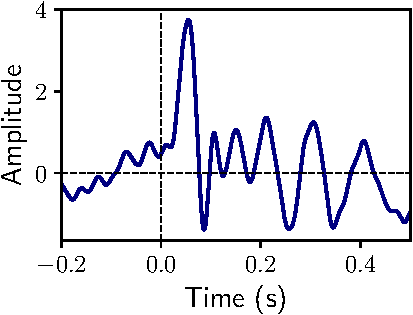
\includegraphics[width=0.3\textwidth]{figures/mvica/camcan_source_0.pdf}%
\raisebox{0.2\height}{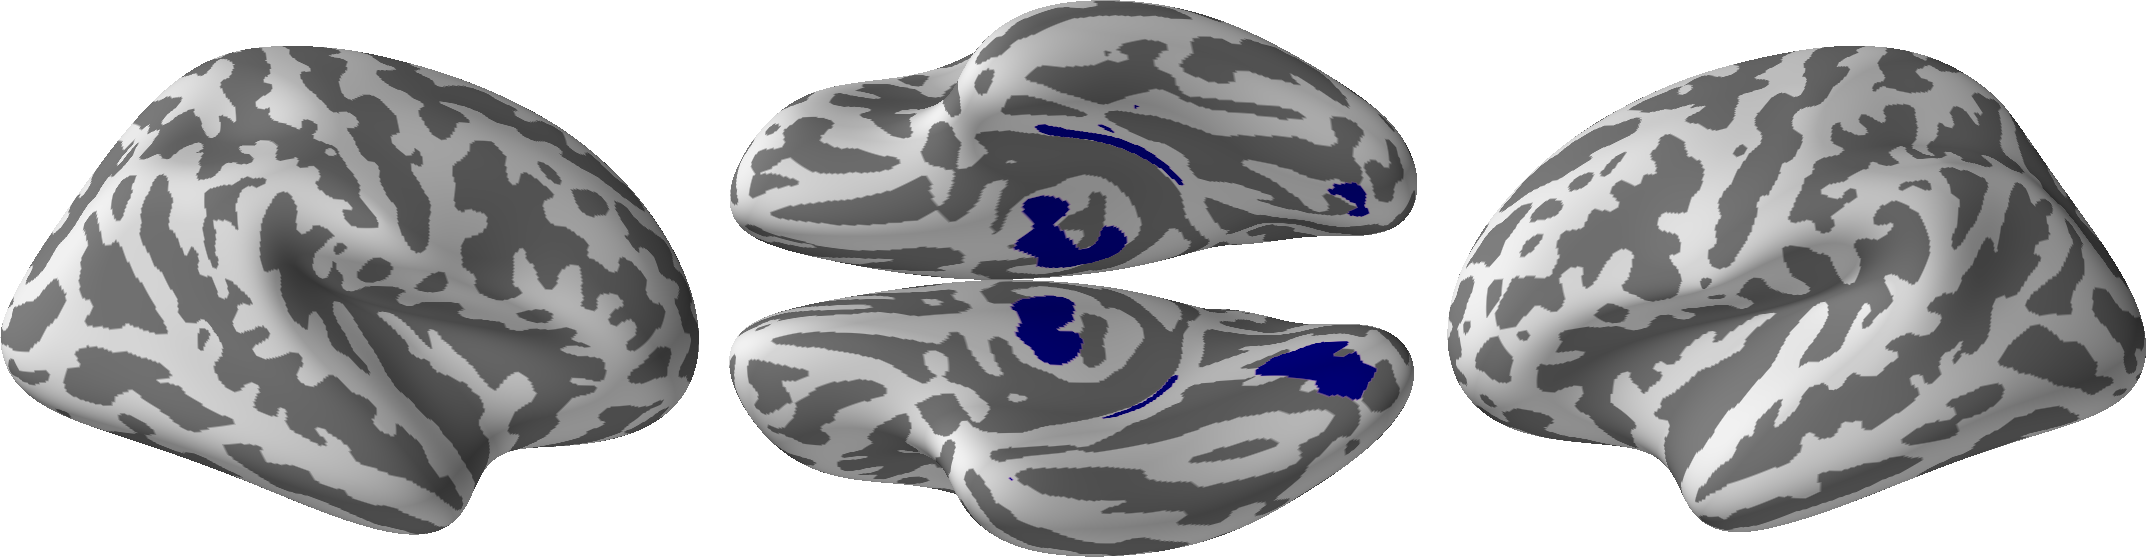
\includegraphics[width=0.68\textwidth]{figures/mvica/montage_0.png}} \\
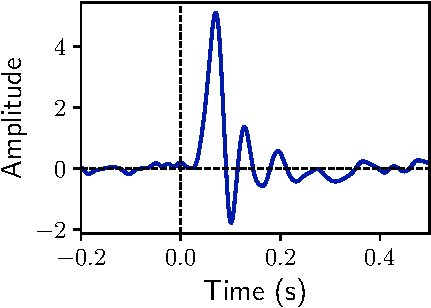
\includegraphics[width=0.3\textwidth]{figures/mvica/camcan_source_1.pdf}%
\raisebox{0.2\height}{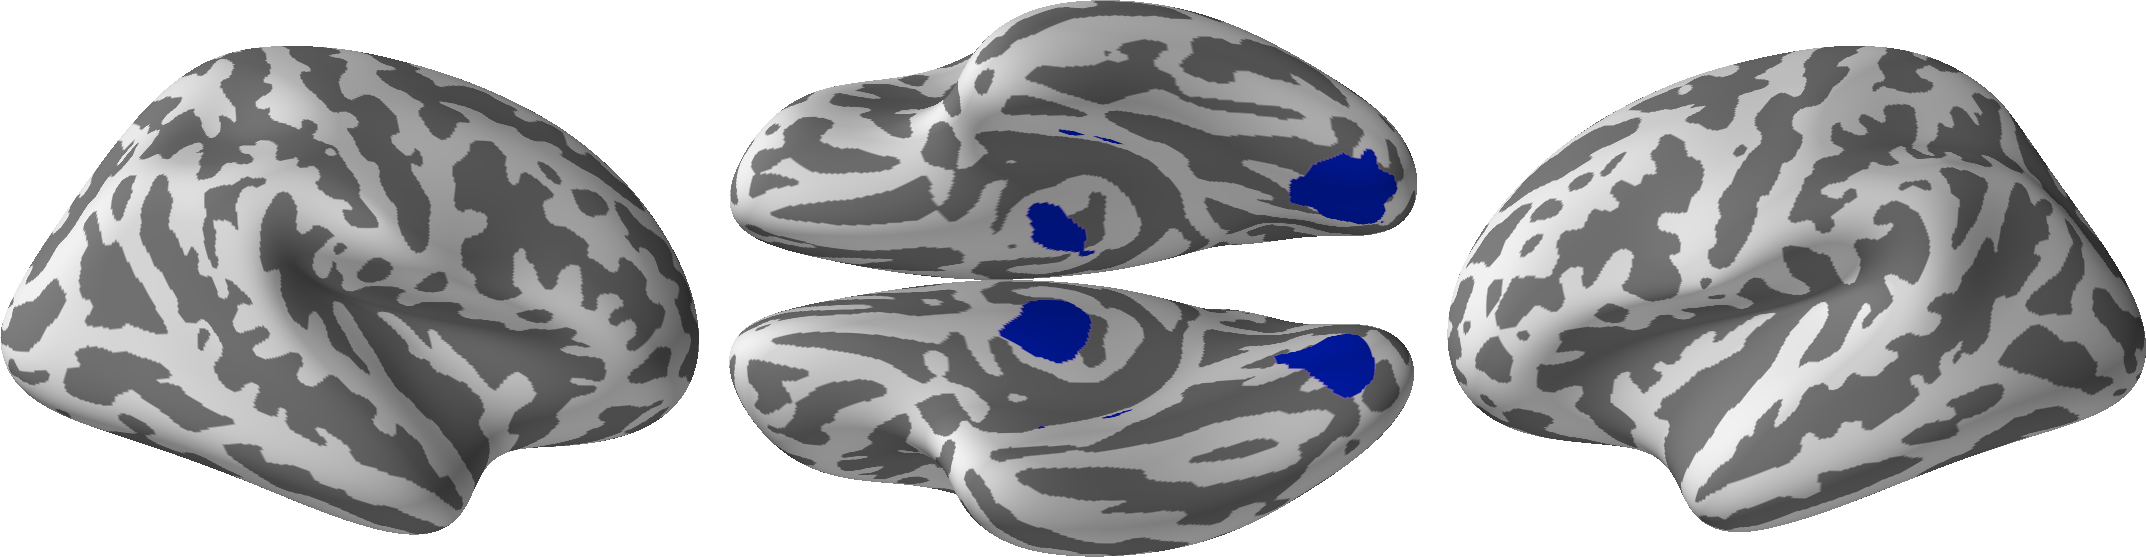
\includegraphics[width=0.68\textwidth]{figures/mvica/montage_1.png}} \\
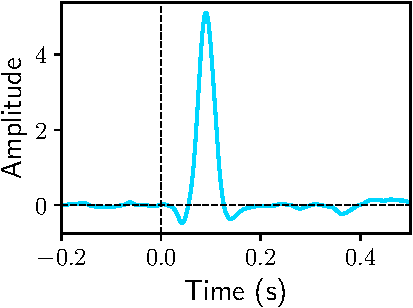
\includegraphics[width=0.3\textwidth]{figures/mvica/camcan_source_2.pdf}%                        
\raisebox{0.2\height}{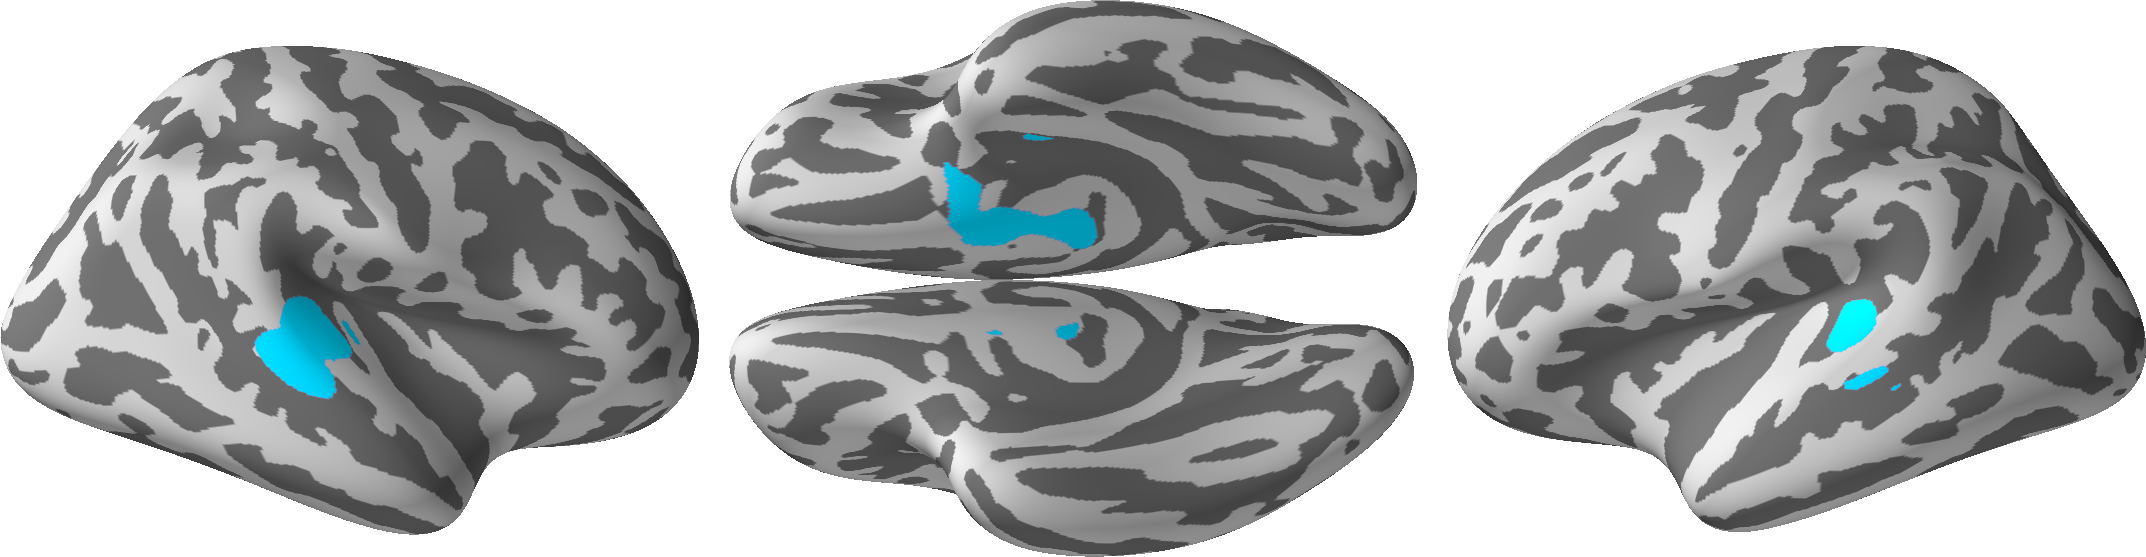
\includegraphics[width=0.68\textwidth]{figures/mvica/montage_2.png}} \\
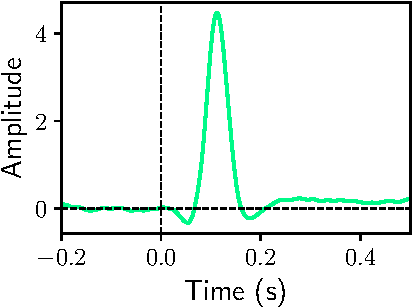
\includegraphics[width=0.3\textwidth]{figures/mvica/camcan_source_3.pdf}%  
\raisebox{0.2\height}{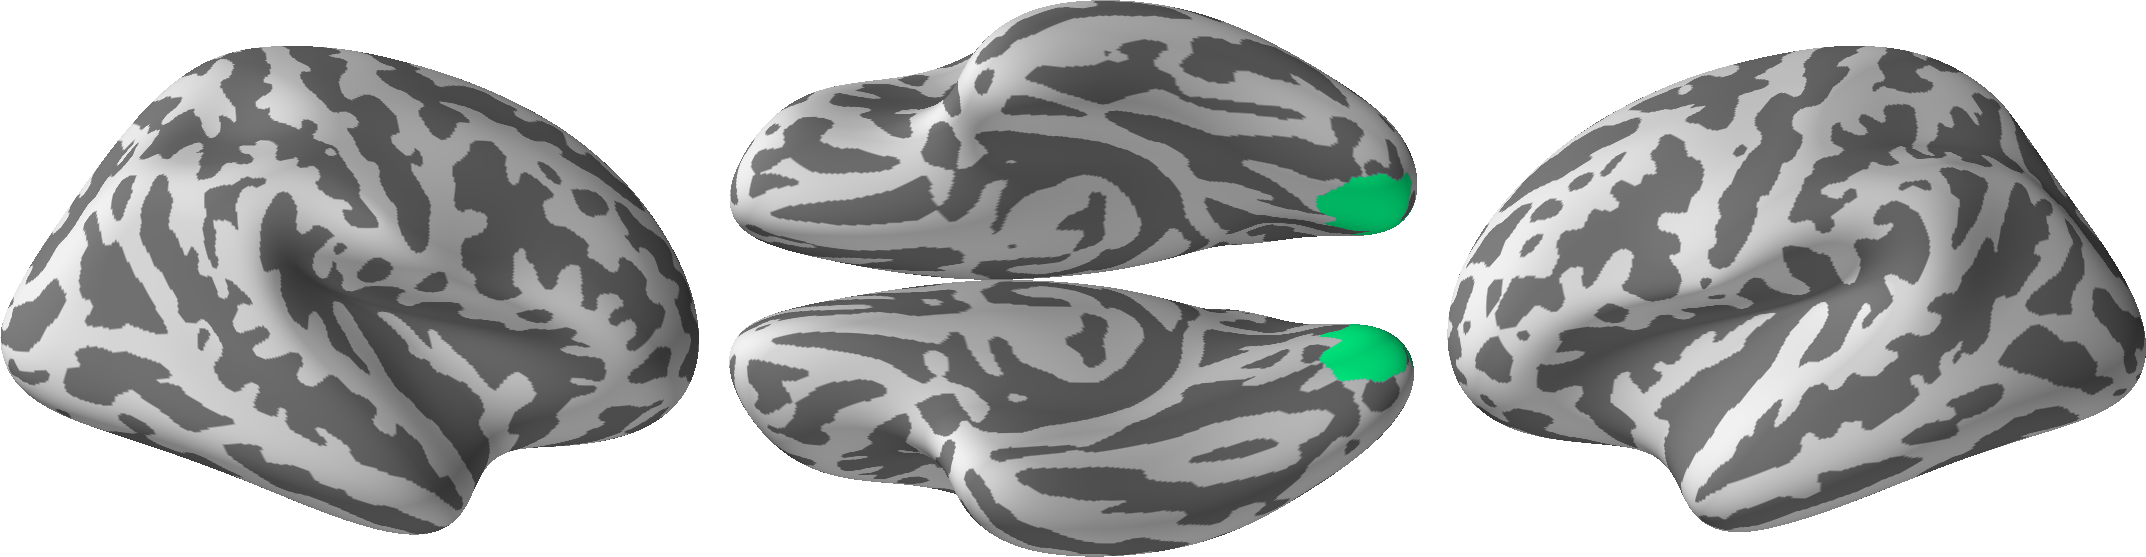
\includegraphics[width=0.68\textwidth]{figures/mvica/montage_3.png}} \\
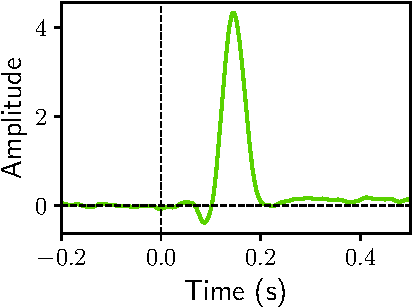
\includegraphics[width=0.3\textwidth]{figures/mvica/camcan_source_4.pdf}%
\raisebox{0.2\height}{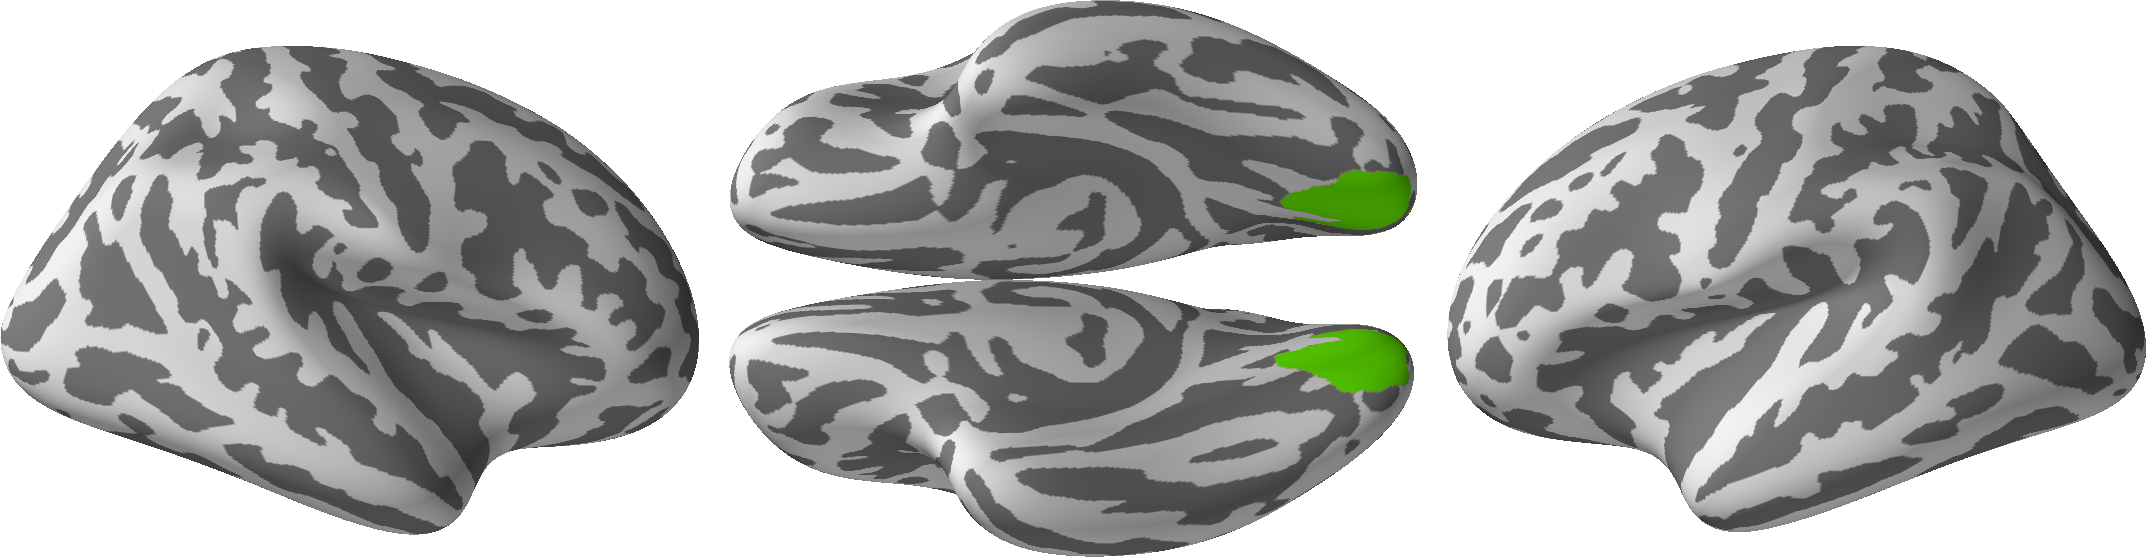
\includegraphics[width=0.68\textwidth]{figures/mvica/montage_4.png}} \\
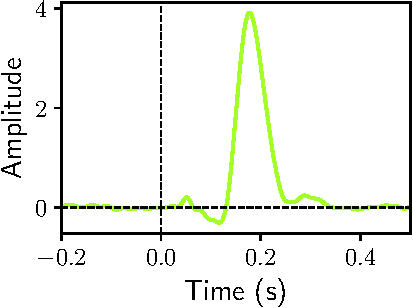
\includegraphics[width=0.3\textwidth]{figures/mvica/camcan_source_5.pdf}%
\raisebox{0.2\height}{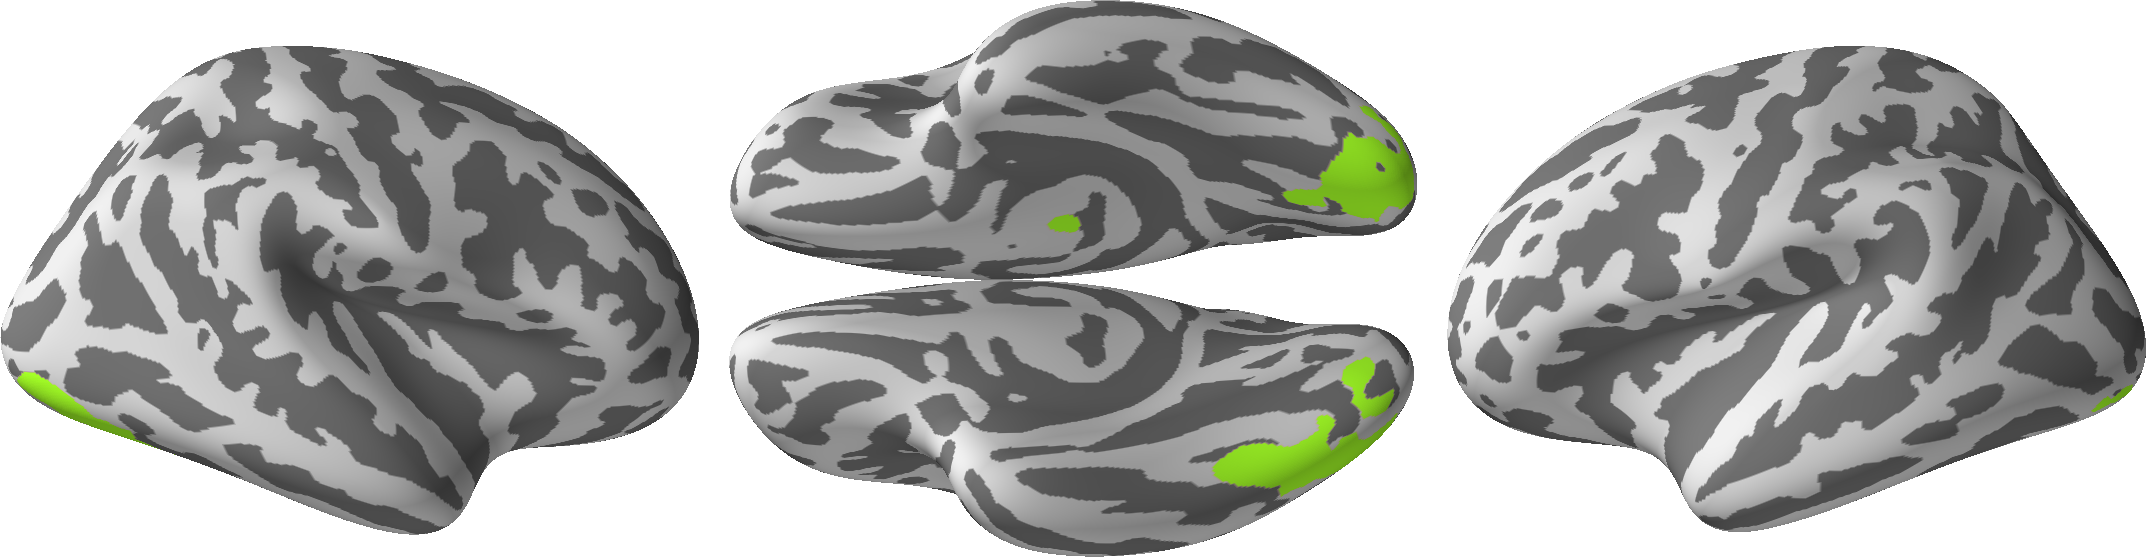
\includegraphics[width=0.68\textwidth]{figures/mvica/montage_5.png}} \\
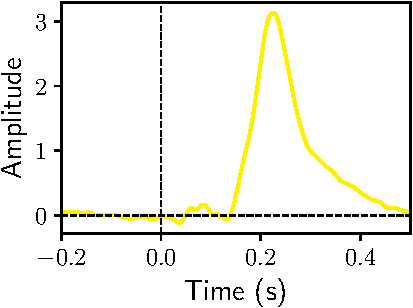
\includegraphics[width=0.3\textwidth]{figures/mvica/camcan_source_6.pdf}%
\raisebox{0.2\height}{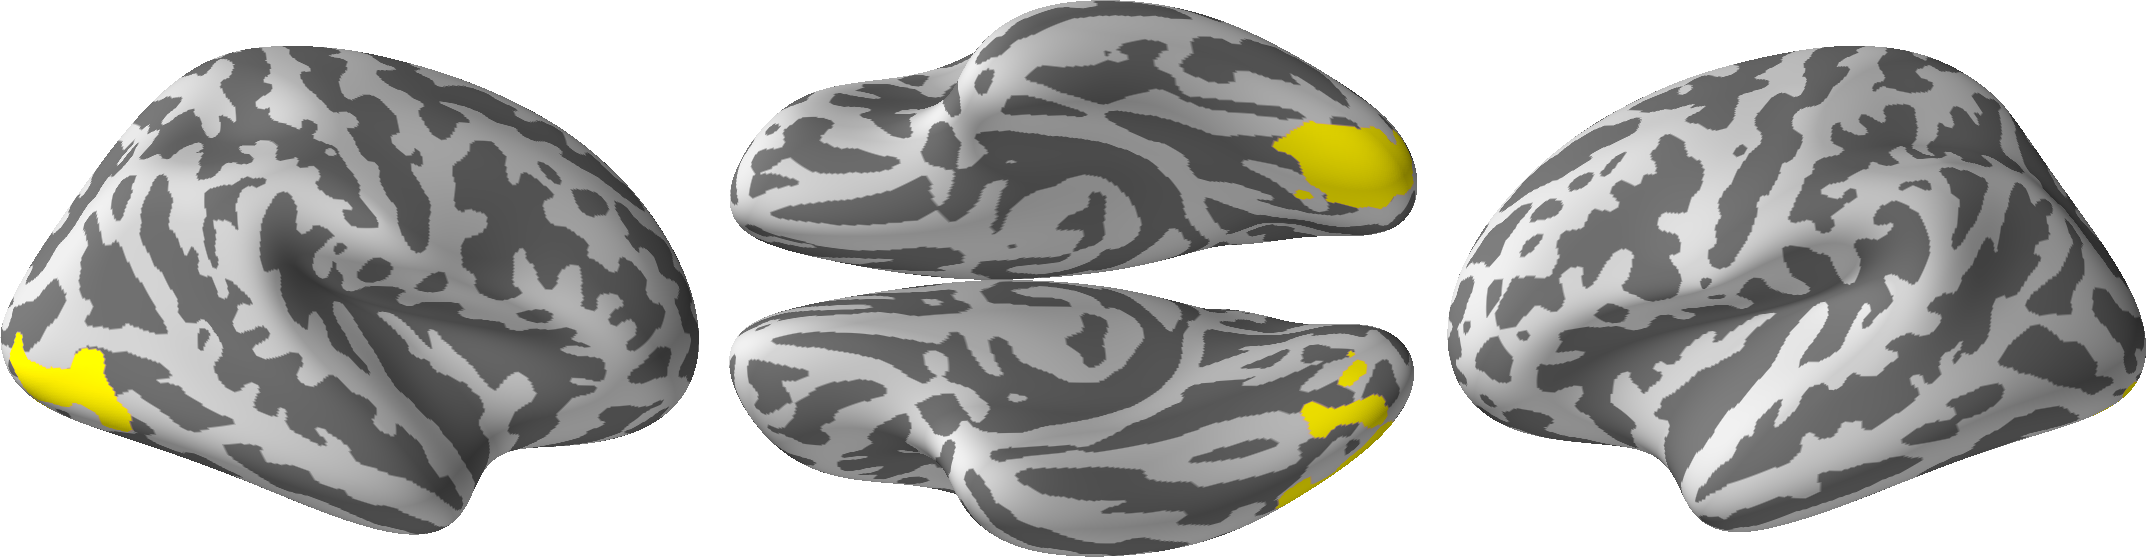
\includegraphics[width=0.68\textwidth]{figures/mvica/montage_6.png}} \\
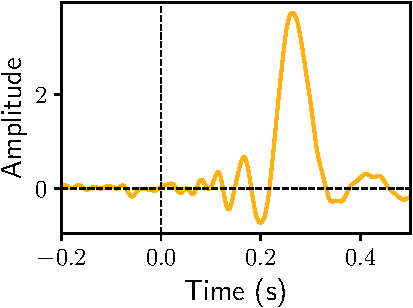
\includegraphics[width=0.3\textwidth]{figures/mvica/camcan_source_7.pdf}%
\raisebox{0.2\height}{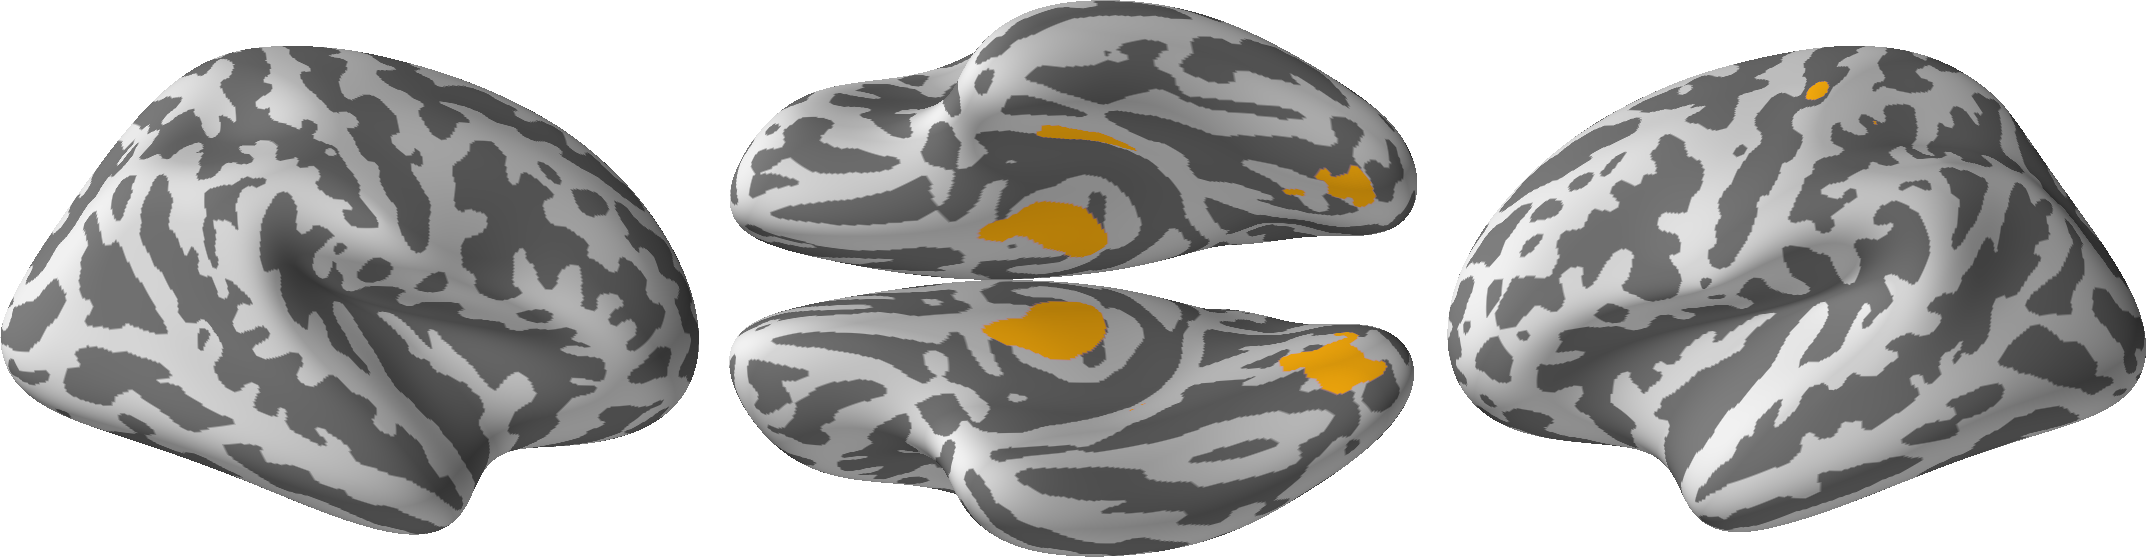
\includegraphics[width=0.68\textwidth]{figures/mvica/montage_7.png}} \\
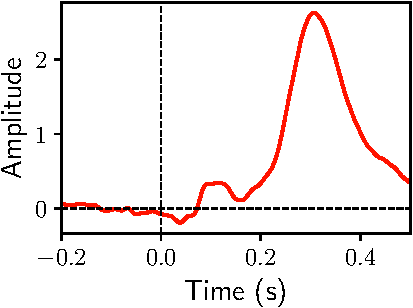
\includegraphics[width=0.3\textwidth]{figures/mvica/camcan_source_8.pdf}%
\raisebox{0.2\height}{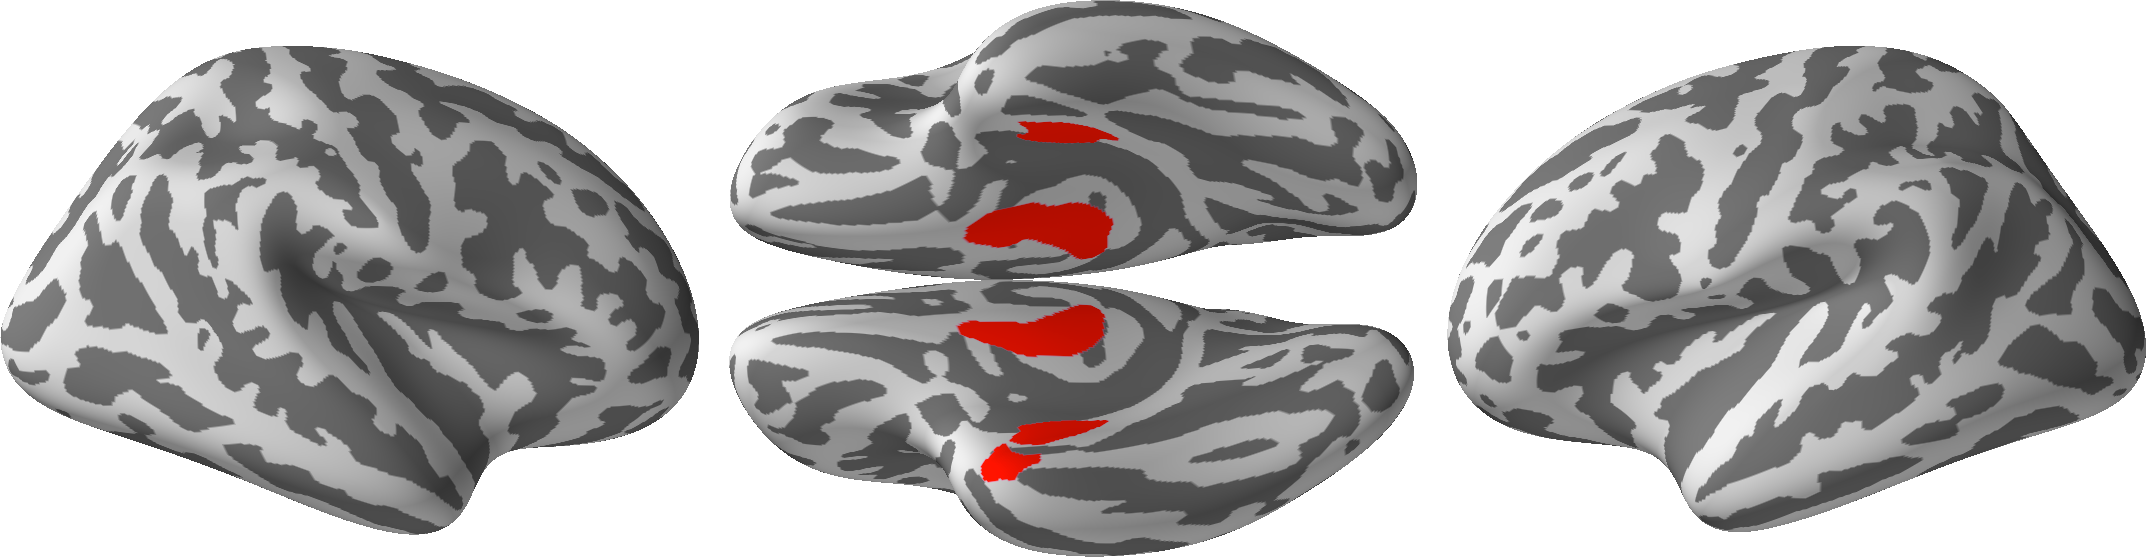
\includegraphics[width=0.68\textwidth]{figures/mvica/montage_8.png}} \\
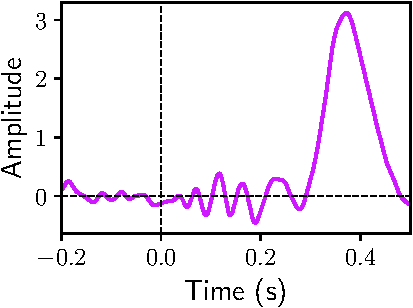
\includegraphics[width=0.3\textwidth]{figures/mvica/camcan_source_9.pdf}%
\raisebox{0.2\height}{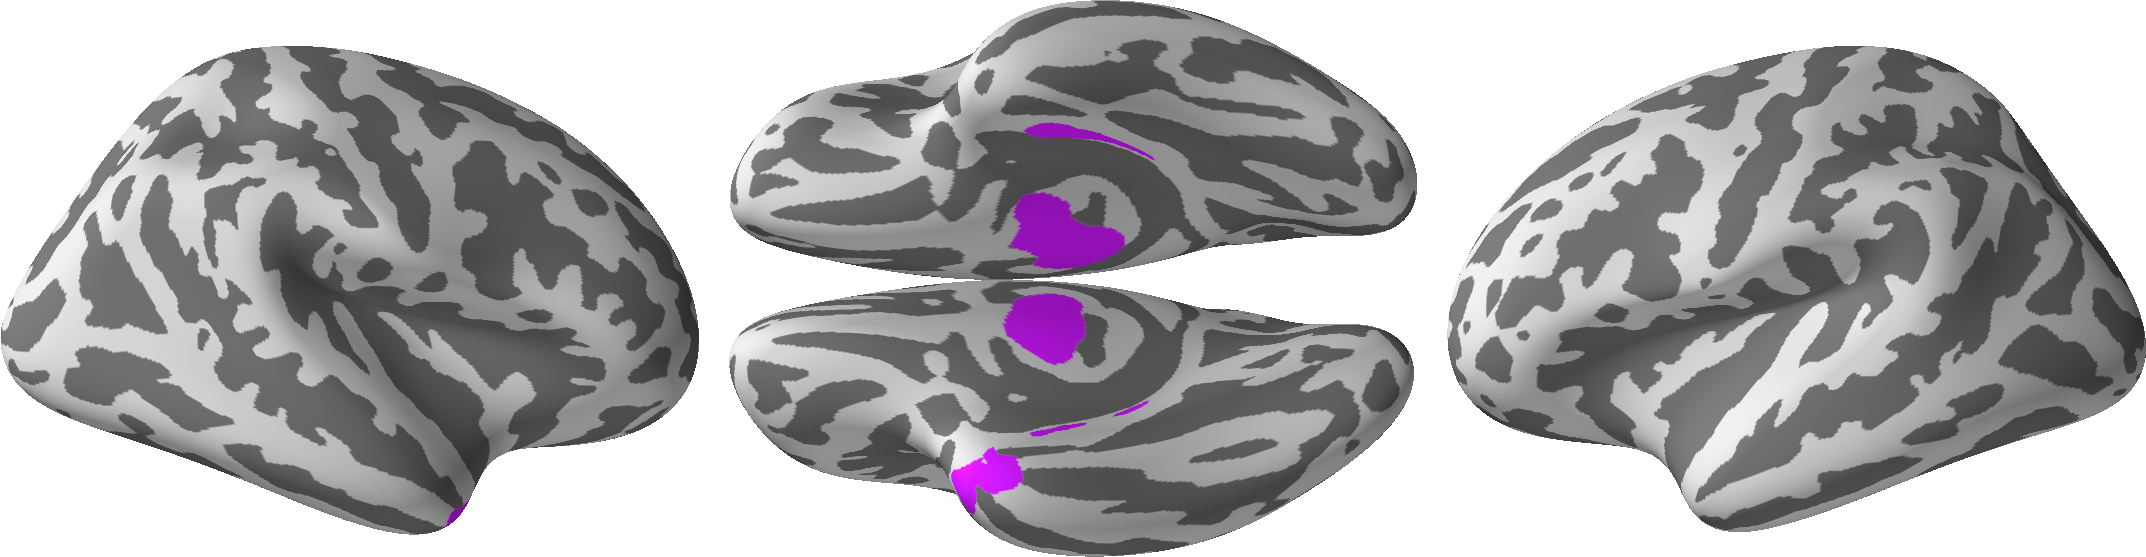
\includegraphics[width=0.68\textwidth]{figures/mvica/montage_9.png}} \\
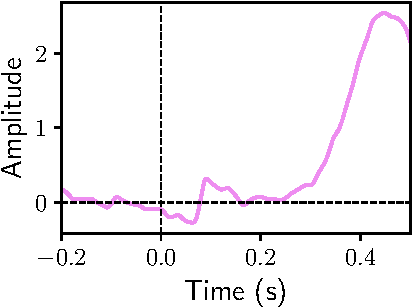
\includegraphics[width=0.3\textwidth]{figures/mvica/camcan_source_10.pdf}%
\raisebox{0.2\height}{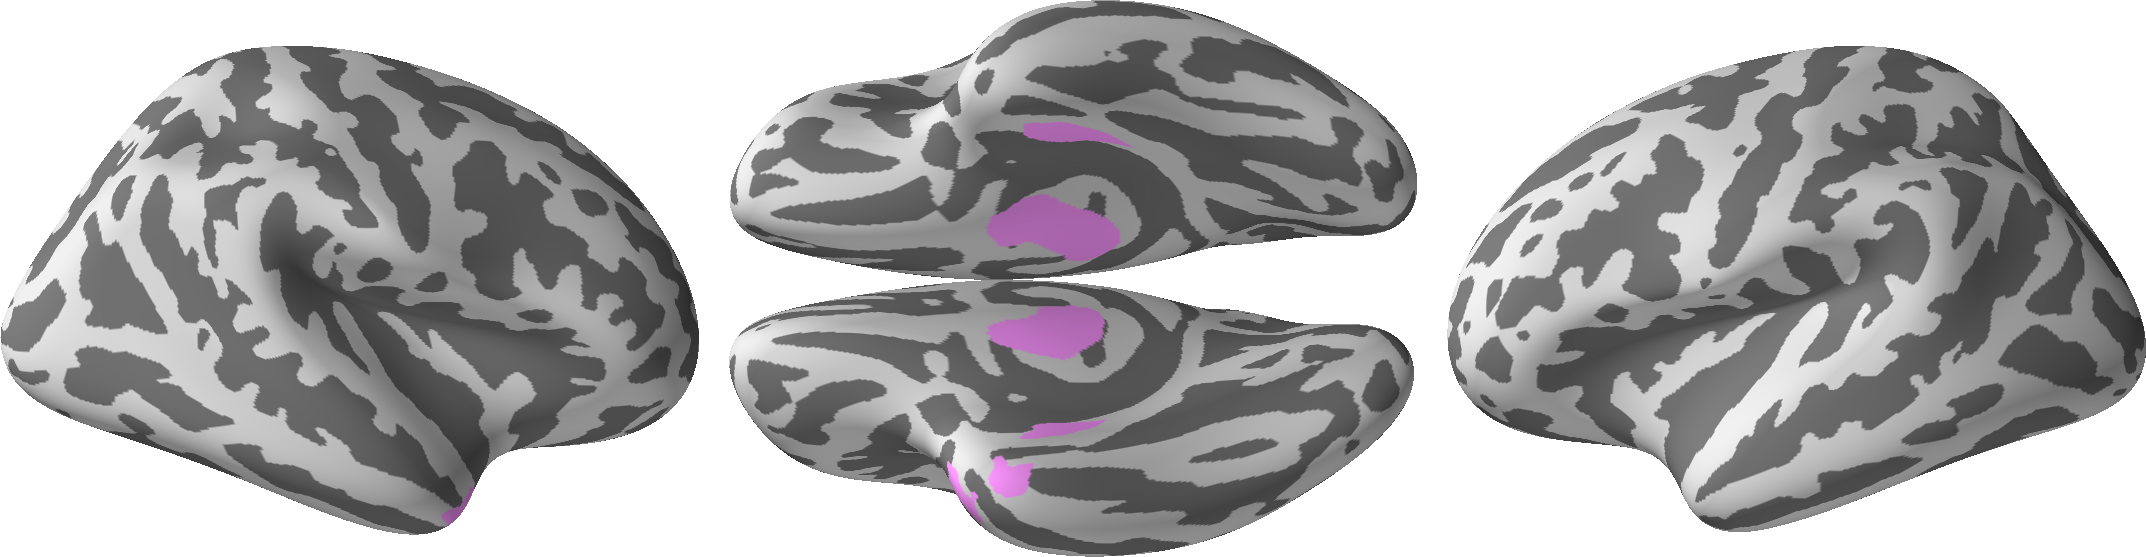
\includegraphics[width=0.68\textwidth]{figures/mvica/montage_10.png}} \\
}

\section{Average forward operators on fMRI datasets}
\label{sec:spatial_maps}
We display the average forward operator across subjects on the Raiders, Forrest, Clips and Sherlock datasets obtained with MultiViewICA and ConcatICA with 5 components. A 5~mm spatial smoothing was applied on all datasets, and the confound signals corresponding to the 5 components with the highest variance were removed before applying MultiViewICA or ConcatICA.

{\centering

  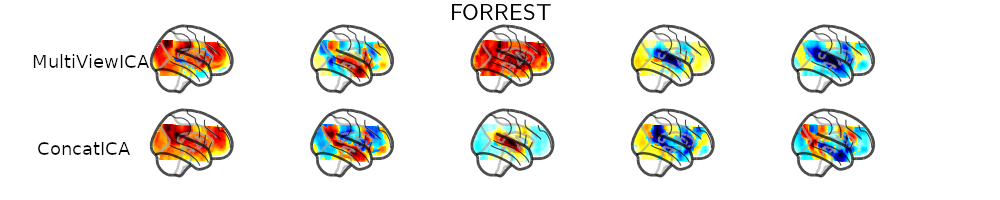
\includegraphics[width=\textwidth]{figures/mvica/maps_forrest.png} \\
  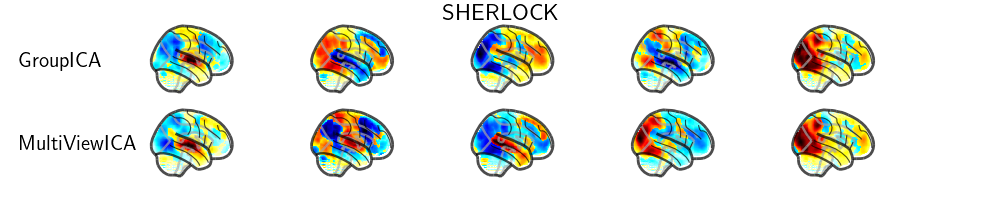
\includegraphics[width=\textwidth]{figures/mvica/maps_sherlock.png} \\
  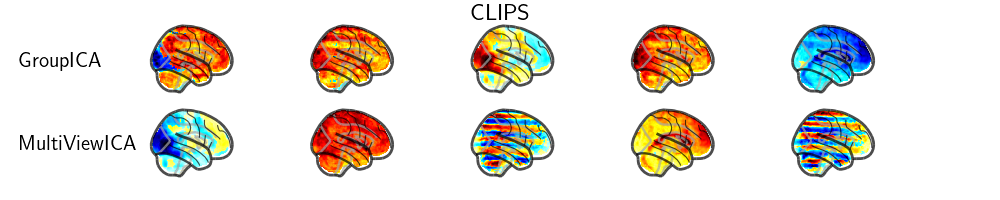
\includegraphics[width=\textwidth]{figures/mvica/maps_gallant.png} \\
  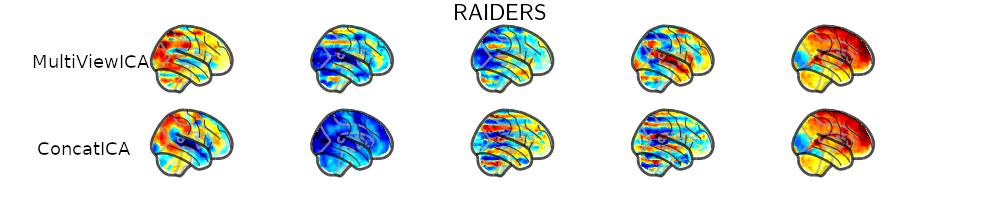
\includegraphics[width=\textwidth]{figures/mvica/maps_raiders.png} \\
}

\section{Synthetic benchmark using additive noise on the sensors}
\label{app:complex_cov}
We generate data according to the model $\xb_i = A_i\sbb + \nb_i$, where $\xb_i \in \mathbb{R}^{50}$, $\sbb \in \mathbb{R}^{20}$, and $\nb_i\sim \mathcal{N}(0, \sigma^2 I_{50})$. After applying individual PCA to obtain signals of dimension $20$, we apply the different ICA algorithms and report the reconstruction error in fig.~\ref{fig:reconstruction_synth}.

\begin{figure}
  \center
  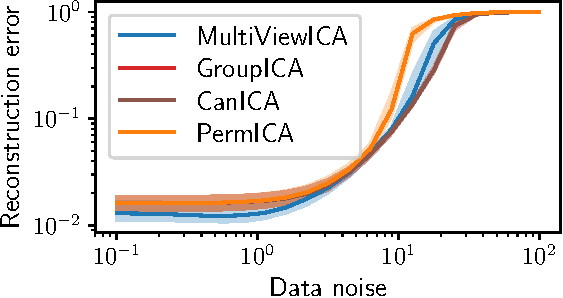
\includegraphics[width=0.5\linewidth]{figures/mvica/distance.pdf}
  \caption{Synthetic experiment with model $\xb_i = A_i\sbb + \nb_i$} %{Light Unit}
  \label{fig:reconstruction_synth}
\end{figure}

\section{Summary of our quantitative results}
\label{sec:app_real_data}
Our quantitative results for the fMRI experiments of time-segment matching and BOLD signal reconstruction and on for the MEG phantom data experiment are summarized, respectively, in Table~\ref{tab:timeseg}, Table~\ref{tab:recon} and Table~\ref{tab:meg}. All methods are compared upon extraction of components with the same dimensionality ($20$ components).

\begin{table}
    \centering
    \begin{tabular}{|c|c | c | c|}
            \hline
         \textbf{Dataset} & \textbf{Method} & \textbf{Accuracy} & \textbf{Confidence interval} \\
         \hline
clips   & Chance      & 0.002&[0.001, 0.003] \\
        & CanICA    & 0.130&[0.112, 0.147] \\
        & PCA + ConcatICA      & 0.124&[0.109, 0.139] \\
        & ConcatICA    & 0.152&[0.133, 0.171] \\

        & PermICA     & 0.147&[0.126, 0.169] \\
        & SRM         & 0.115&[0.104, 0.126] \\
        & MultiViewICA& \textbf{0.167}&[0.142, 0.192] \\
        \hline
forrest & Chance      & 0.002&[0.001, 0.002] \\
        & CanICA    & 0.192&[0.170, 0.214] \\
        & PCA + ConcatICA      & 0.088&[0.077, 0.098] \\
        & ConcatICA    & 0.154&[0.137, 0.170] \\
        & PermICA     & 0.135&[0.118, 0.152] \\
        & SRM         & 0.188&[0.173, 0.203] \\
        & MultiViewICA& \textbf{0.448}&[0.411, 0.484] \\
        \hline
raiders & Chance      & 0.002&[0.001, 0.003] \\
        & CanICA    & 0.256&[0.220, 0.291] \\
        & PCA + ConcatICA      & 0.331&[0.289, 0.372] \\
        & ConcatICA    & 0.321&[0.281, 0.361] \\
        & PermICA     & 0.381&[0.341, 0.421] \\
        & SRM         & 0.265&[0.240, 0.289] \\
         & MultiViewICA& \textbf{0.408}&[0.358, 0.458] \\
         \hline
sherlock& Chance      & 0.005&[0.003, 0.006] \\
        & CanICA    & 0.607&[0.567, 0.648] \\
        & PCA + ConcatICA      & 0.454&[0.416, 0.492] \\
        & ConcatICA    & 0.519&[0.481, 0.556] \\
        & PermICA     & 0.399&[0.365, 0.434] \\
        & SRM         & 0.493&[0.465, 0.520] \\
        & MultiViewICA& \textbf{0.873}&[0.844, 0.903] \\
\hline
    \end{tabular}
    \caption{Timesegment matching: Summary of our quantitative results. We report the mean accuracy across cross-validation splits.}
    \label{tab:timeseg}
\end{table}

\begin{table}
    \centering
    \begin{tabular}{|c|c | c | c|}
            \hline
         \textbf{Dataset} & \textbf{Method} & \textbf{R2 score} & \textbf{Confidence interval} \\
         \hline
         clips   & Chance              & 0.000&[0.000 ,0.000] \\
        & CanICA            &  0.110&[ 0.097 , 0.123] \\
        & PCA + ConcatICA              &  0.075&[ 0.058 , 0.092] \\
        & ConcatICA            &  0.077&[ 0.059 , 0.094] \\
        & PermICA             &  0.099&[ 0.087 , 0.111] \\
        & SRM                 &  0.081&[ 0.069 , 0.094] \\
        & MultiViewICA        &  \textbf{0.114}&[ 0.099 , 0.128] \\
        \hline
forrest & Chance              & 0.000&[0.000 ,0.000] \\
        & CanICA            &  0.181&[ 0.169 , 0.193] \\
        & PCA + ConcatICA              &  0.072&[ 0.054 , 0.090] \\
        & ConcatICA            &  0.081&[ 0.062 , 0.099] \\
        & PermICA             &  0.098&[ 0.090 , 0.106] \\
        & SRM                 &  0.180&[ 0.168 , 0.193] \\
        & MultiViewICA        &  \textbf{0.191}&[ 0.177 , 0.204] \\
        \hline
raiders & Chance              & 0.000&[0.000 ,0.000] \\
        & CanICA            &  0.136&[ 0.122 , 0.149] \\
        & PCA + ConcatICA              &  0.063&[ 0.045 , 0.080] \\
        & ConcatICA            &  0.062&[ 0.043 , 0.081] \\
        & PermICA             &  0.107&[ 0.091 , 0.124] \\
        & SRM                 &  0.138&[ 0.121 , 0.154] \\
        & MultiViewICA        &  \textbf{0.144}&[ 0.124 , 0.164] \\
        \hline
sherlock& Chance              & 0.000&[0.000 ,0.000] \\
        & CanICA            &  0.156&[ 0.141 , 0.172] \\
        & PCA + ConcatICA              &  0.087&[ 0.065 , 0.108] \\
        & ConcatICA            &  0.091&[ 0.070 , 0.112] \\
        & PermICA             &  0.067&[ 0.055 , 0.078] \\
        & SRM                 &  \textbf{0.164}&[ 0.147 , 0.181] \\
        & MultiViewICA        &  0.161&[ 0.142 , 0.180] \\
        \hline

         
    \end{tabular}
    \caption{Reconstructing the BOLD signal of missing subjects: Summary of our quantitative results. We report the mean R2 score across cross-validation splits.}
    \label{tab:recon}
\end{table}

\begin{table}
    \centering
    \begin{tabular}{|c|c|c|c}
    \hline
         \textbf{Method} & \textbf{Reconstruction error} & \textbf{1st and 3d quartiles} 
         \\
         \hline
         MultiViewICA & \textbf{0.0045} & [0.0039, 0.0052] \\ 
ConcatICA & 0.1098 & [0.0549, 0.1734] \\ 
PCA+ConcatICA & 0.1111 & [0.0760, 0.1502] \\ 
PermICA & 0.0730 & [0.0423, 0.1037] \\ 
\hline
    \end{tabular}
    \caption{Phantom MEG data: Summary of our quantitative results with 2 epochs. We report the median reconstruction error across cross-validation splits.}
    \label{tab:meg}
\end{table}

